\documentclass[10pt]{article}
\usepackage[margin=0.78in]{geometry}
\usepackage{amsmath,amssymb,booktabs,array,microtype}
\usepackage{xcolor,hyperref,graphicx,tikz}
\usetikzlibrary{arrows.meta,positioning,fit}
\hypersetup{colorlinks=true,linkcolor=blue!55!black,citecolor=blue!55!black,urlcolor=blue!55!black}
\definecolor{echocyan}{HTML}{0891B2}
\definecolor{frebamber}{HTML}{D97706}
\newcommand{\method}{\textsc{ECHO-CAVER}}
\title{\texttt{[Research]} ECHO-CAVER: Evidence-Tangent Residual Readers\\for Frozen Visual-Comparison Carriers}
\author{JaeWoo Choi\\Private research archive}
\date{24 August 2026}

\begin{document}
\maketitle

\begin{abstract}
FREB-CAVER inserts query-reference comparison evidence into a frozen JUDO
multimodal reasoner, but the frozen downstream decoder may not optimally read
the new state. We introduce \method, a parameter-efficient writer-reader
alignment mechanism. Rank-16 LoRA readers are placed immediately after five
FREB evidence writers, and their output directions are constrained to the
rank-32 left-singular span of the corresponding frozen writer. Gradient and
post-optimizer projection preserve the constraint, while zero initialization
provides exact FREB identity. On a Full-MMAD-compatible 39,670-question census,
\method obtains 82.416847\% strict normalized 28-cell Overall. This is
descriptively +1.216847 points over JUDO's paper-reported 81.20\% and +0.126847
points over AD-Copilot-Thinking's reported 82.29\% \cite{kang2026judo,jiang2026adcopilot}.
These are cross-paper comparisons rather than paired re-evaluations. On a 5,600-row
query-reference-component-disjoint paired panel, the point estimate improves
by 0.2698 points, but the cluster-bootstrap 95\% interval
[-0.0937, 0.6317] includes zero and exact McNemar $p=0.1332$. The archive thus
supports a benchmark-level positive signal, not a confirmed generalization
claim. Code, the 9.1MB adapter, strict analyzers, and sealed receipts are
included without redistributing MMAD or JUDO.
\end{abstract}

\section{Introduction}
Industrial anomaly question answering couples fine-grained visual comparison
with domain-oriented language reasoning. MMAD defines seven such tasks across
four industrial sources \cite{jiang2024mmad}; JUDO improves this setting by
juxtaposing a query with normal context and training domain reasoning
\cite{kang2026judo}. FREB-CAVER adds a model-native comparison carrier to the
frozen JUDO decoder \cite{frebcaver2026}.

The remaining problem is a hidden-state interface mismatch. FREB writes a new
visual signal, whereas the downstream JUDO blocks remain optimized for their
original state distribution. Unconstrained fine-tuning could teach those
blocks to read the signal but risks opening language-only directions and
forgetting previously correct behavior. \method instead derives its trainable
geometry from the frozen carrier itself.

Our contribution is a causal writer-reader placement rule, an evidence-tangent
LoRA constraint applied to both gradients and post-Adam weights, and a
fail-closed evaluation archive that separates full-benchmark behavior from
component-disjoint generalization evidence.

\section{Method}
\subsection{Evidence-tangent readers}
Let the $i$th frozen FREB writer inject through
$W_i\in\mathbb{R}^{d\times h}$ at decoder layer $\ell_i$. From
$W_i=U_i\Sigma_iV_i^\top$, we retain $U_{i,k}$ for $k=32$ and define
$P_i=U_{i,k}U_{i,k}^\top$. A rank-$r$ LoRA reader at layer $\ell_i+1$ is
\begin{equation}
 y=W_0x+\frac{\alpha}{r}B_iA_ix,\qquad r=16,\quad\alpha=32.
\end{equation}
Its trainable output matrix is constrained by
\begin{equation}
 \nabla B_i\leftarrow P_i\nabla B_i,\qquad
 B_i\leftarrow P_iB_i
\end{equation}
during backpropagation and after every AdamW step. This differs from
orthogonal-subspace continual learning \cite{wang2023olora}: ECHO learns
inside the existing evidence span instead of reserving a new orthogonal task
subspace.

\begin{figure*}[t]
\centering
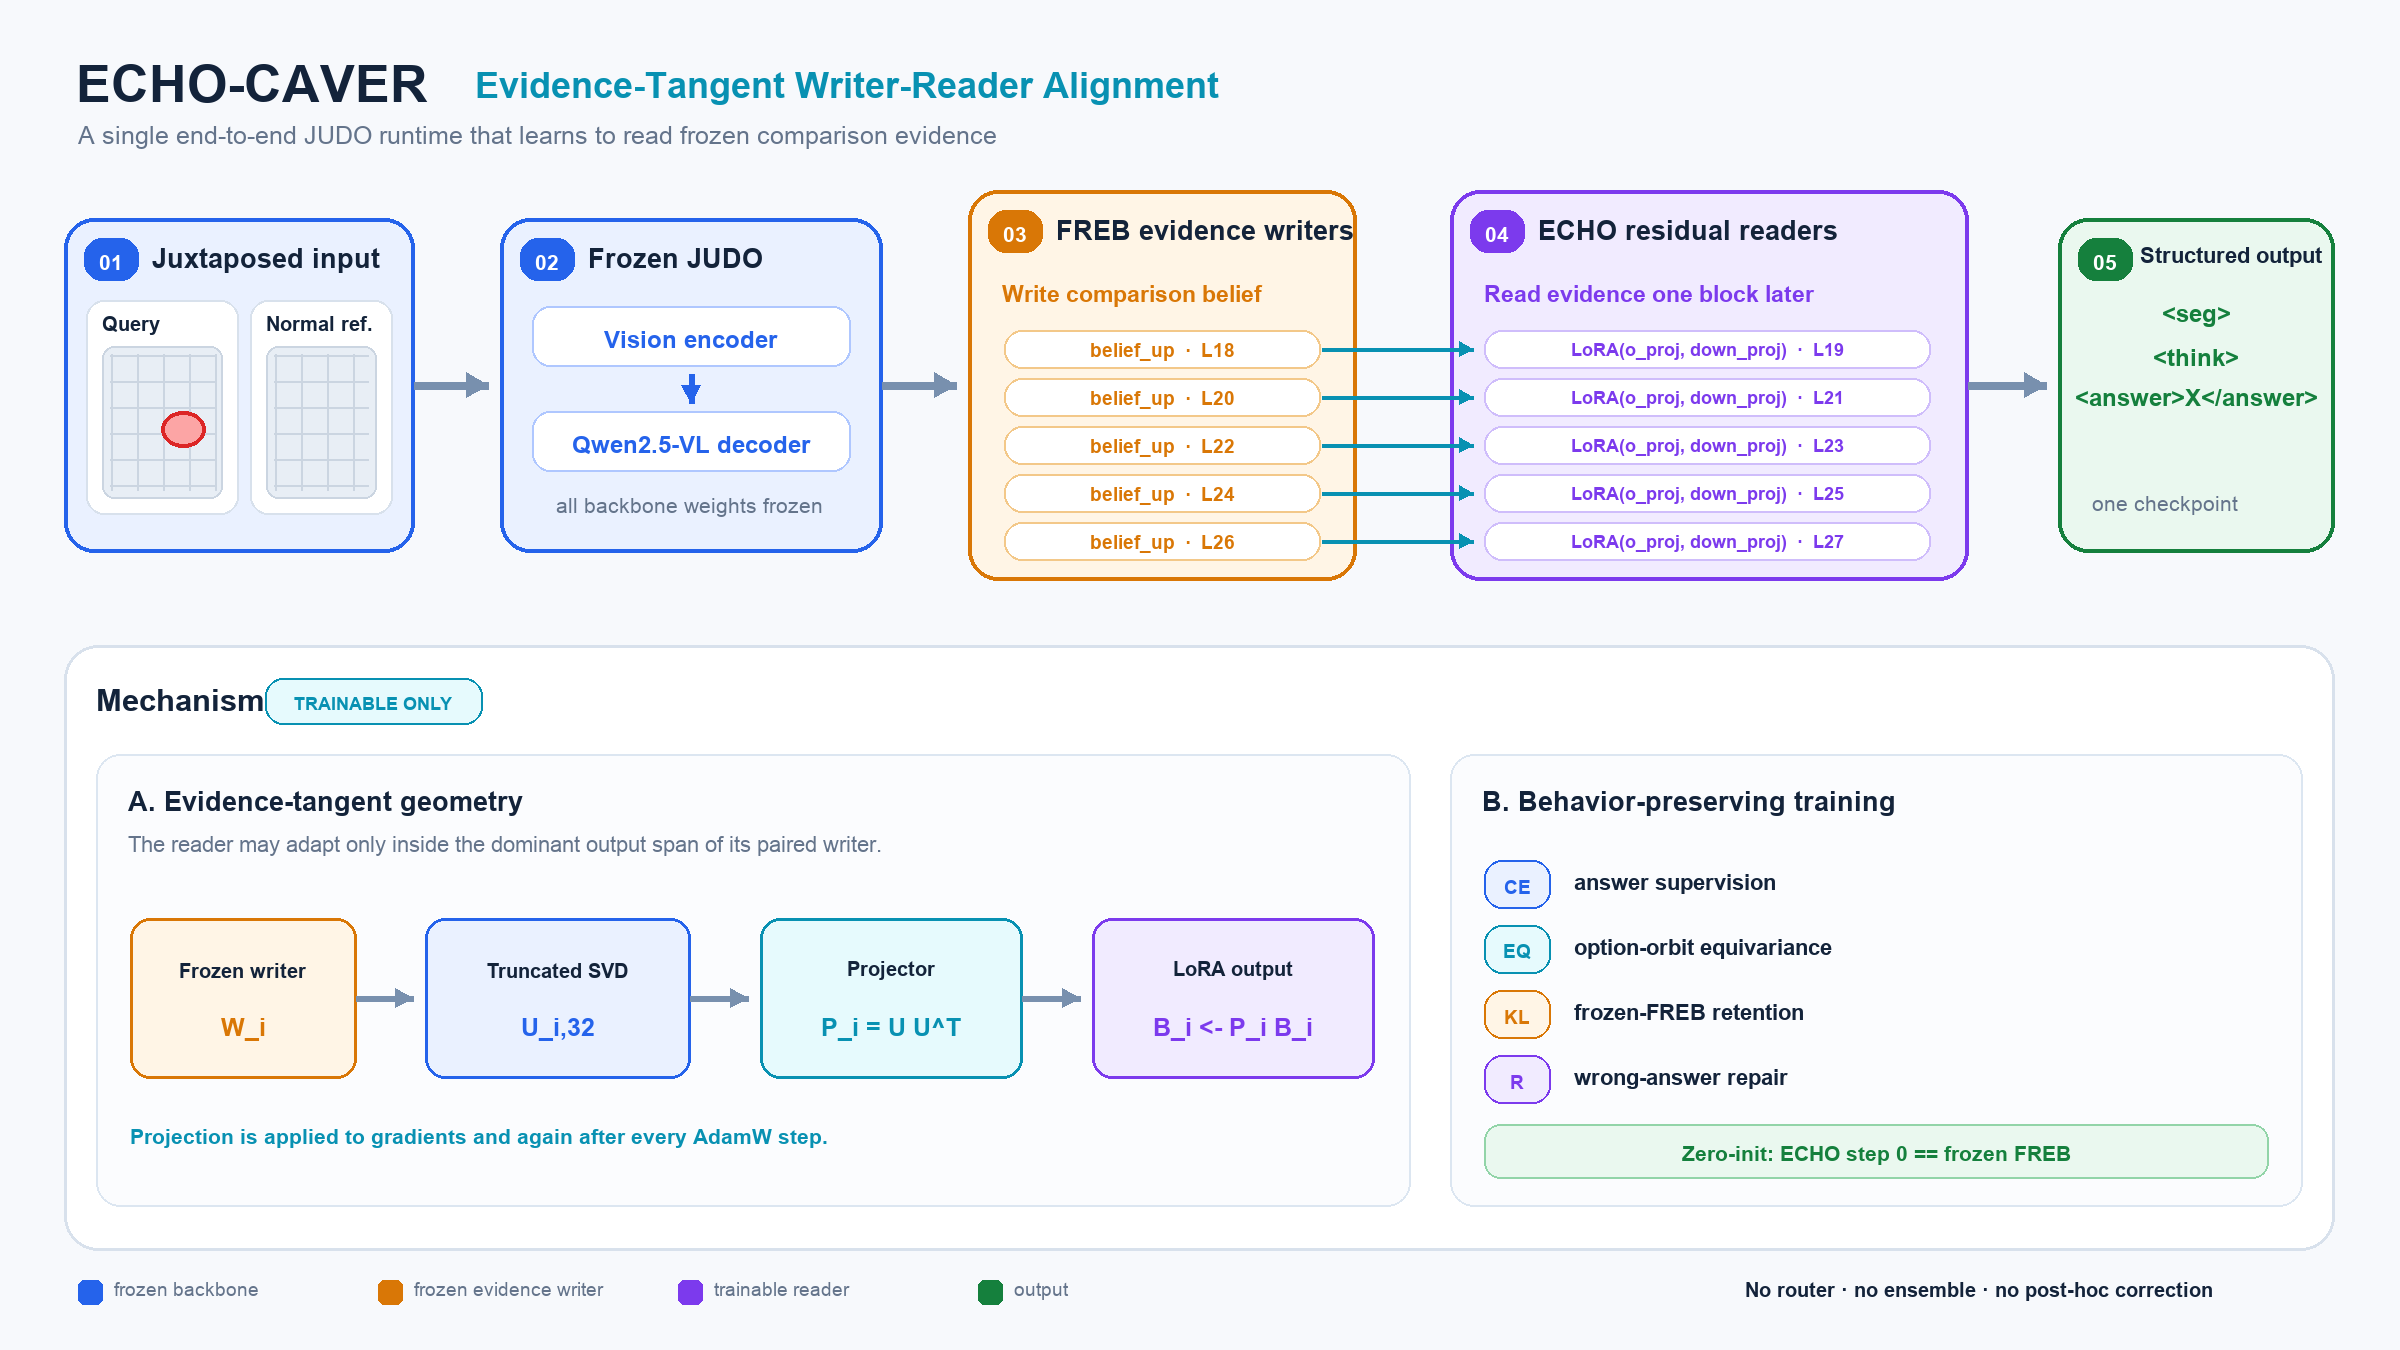
\includegraphics[width=\textwidth]{../assets/echo_caver_architecture.png}
\caption{ECHO-CAVER architecture. Frozen JUDO and FREB components are separated
from trainable evidence-tangent readers. Each reader is placed one block after
its paired writer and constrained to the writer's rank-32 output span.}
\label{fig:architecture}
\end{figure*}

\subsection{Objective}
Training pairs each question with a semantic option permutation. For candidate
logits $z$, frozen-FREB logits $z_0$, and target $y$, the loss is
\begin{equation}
\mathcal{L}=\mathcal{L}_{\mathrm{CE}}+0.25\mathcal{L}_{\mathrm{equiv}}
+1.0\,\mathrm{KL}(p_0\|p)+0.75\mathcal{L}_{\mathrm{repair}}(m=0.25).
\end{equation}
The repair term reverses a frozen-FREB wrong-answer ranking. Zero-initialized
LoRA-B matrices make the pre-update model exactly equal to FREB.

\section{Training protocol}
JUDO and FREB are frozen. We train 2,375,680 parameters (0.02853\% of 8.328B)
on 963 non-AD option-orbit pairs, validate on 184 pairs, and run 100 AdamW steps
with two pairs per batch, learning rate $2\times10^{-5}$, zero weight decay,
and seed 20260824. Training takes 183.07 seconds on one NVIDIA H200 and peaks at
23.84GiB allocated memory. The adapter is 9.1MB.

\section{Evaluation protocol}
The score is the mean of 28 source-by-task cells. Each Anomaly Detection cell
uses label-balanced accuracy; the other cells use accuracy. A completion must
contain exactly one valid case-sensitive answer tag. Invalid completions are
incorrect. Full evaluation is an exact eight-shard cover of 39,670 IDs.

The clean panel contains 200 rows in every cell and excludes all
query-reference connected components intersecting training assets. We use an
exact paired McNemar test and 50,000-replicate component-cluster bootstrap.

\section{Results}
\begin{table}[t]
\centering
\caption{MMAD standard 1-shot comparison. JUDO and AD-Copilot values are
paper-reported; ECHO is the strict 39,670-row census in this archive.}
\resizebox{\textwidth}{!}{%
\begin{tabular}{lrrrrrrrr}
\toprule
Model & AD & DC & DL & DD & DA & OC & OA & Overall \\
\midrule
JUDO \cite{kang2026judo} & 65.04 & 74.74 & 73.01 & 84.56 & 89.41 & 94.04 & 87.58 & 81.20 \\
AD-Copilot \cite{jiang2026adcopilot} & 73.64 & 67.89 & 64.08 & 80.60 & 85.91 & 91.06 & 87.78 & 78.71 \\
AD-Copilot-Thinking \cite{jiang2026adcopilot} & \textbf{73.95} & 74.29 & \textbf{76.40} & 84.92 & 86.93 & 91.86 & 87.67 & 82.29 \\
\textbf{ECHO-CAVER v1} & 65.8231 & \textbf{76.7698} & 75.3531 & \textbf{86.1556} & \textbf{89.6094} & \textbf{95.1548} & \textbf{88.0521} & \textbf{82.4168} \\
\bottomrule
\end{tabular}
}
\label{tab:full}
\end{table}

The full run records 32,391/39,670 correct generations, 85.1825\% non-AD
macro, 65.6475\% pooled AD balanced accuracy, and 99.8866\% strict answer
validity. ECHO is numerically +1.216847 points over JUDO and +0.126847 points
over AD-Copilot-Thinking in Overall. External paper rows were not re-scored
with ECHO's exact parser, so these are descriptive cross-paper deltas and not
paired significance estimates.

\begin{table}[t]
\centering
\caption{5,600-row clean paired panel.}
\begin{tabular}{lrrr}
\toprule
Metric & FREB & ECHO & $\Delta$ \\
\midrule
Overall & 80.8060 & 81.0758 & +0.2698 \\
non-AD macro & 83.7292 & 84.0417 & +0.3125 \\
AD balanced accuracy & 62.9112 & 62.8450 & -0.0662 \\
ITT correct & 4556 & 4572 & +16 \\
\bottomrule
\end{tabular}
\label{tab:clean}
\end{table}

There are 58 ECHO-only and 42 FREB-only correct outcomes. Exact McNemar
$p=0.1332$; the cluster-bootstrap Overall delta interval is
[-0.0937,0.6317] points. The clean evidence is positive but inconclusive.

\section{Analysis and limitations}
The full score crosses the archive's 82\% candidate threshold, but it is not a
clean generalization estimate because benchmark-targeted/training-overlap
components are present. JUDO and AD-Copilot use the same task semantics and
standard 1-shot setting, but parser, checkpoint, preprocessing, manifest
cardinality, and aggregation details may differ. The clean panel remains
primary evidence for architecture-level generalization.

ECHO changes reasoning tokens on 1,349/5,600 clean examples, showing that the
evidence-span constraint does not guarantee answer-stage locality. Forty-five
full-run generations are strict-format invalid, compared with nine in the
archived FREB analysis. A successor should combine evidence-tangent readers
with FREB's answer-prefix causal mask.

\section{Reproducibility and ethics}
The archive includes the exact training and inference sources, checkpoint,
strict analyzers, machine-readable metrics, runtime attestations, and SHA-256
identities. It excludes MMAD images and annotations, JUDO weights, FREB weights,
and raw generations. This model is research software and is not validated for
production inspection or safety-critical decisions.

\section{Conclusion}
\method provides a compact mechanism for teaching a frozen decoder to read an
existing multimodal evidence carrier without granting an unconstrained residual
channel. Full-benchmark results motivate retention, while clean paired evidence
requires further replication. The combination of geometric model design and
explicit claim boundaries is the central outcome of this archive.

\bibliographystyle{plain}
\bibliography{references}
\end{document}
